\section{Methods}\label{sec:Methods}
In this section we describe the methods used to model biodiversity at the community level. We first outline our major contribution---a pipeline for spatial biodiversity modeling---and then describe the data, model selection process, and evaluation metrics used in our study.
\subsection{Spatial Biodiversity Modeling Pipeline}\label{subsec:pipeline}
% Rename section to something with spatial biodiversity pipeline
% Was built on Jakob's pipeline and cite. 
The spatial biodiversity modeling pipeline, hereafter referred to as the SBM pipeline, we developed is based on the work of Nyström \parencite{nystrom2024}, and consists of the following three main components: data processing, feature engineering, and model training. We designed the SBM-pipe to be flexible in terms of the types of data and models that can be used, allowing for a wide range of applications in biodiversity modeling. The goal of the SBM pipeline is to facilitate the development and evaluation of top-down community-level biodiversity models, and to provide a tool for ecologists and researchers to explore the potential of these models in predicting biodiversity patterns and trends. The pipeline is implemented in Python along with a configuration file and for each component is available on GitHub \parencite{sbm-pipe}, allowing for easy access and collaboration among researchers in the field of biodiversity modeling. A diagram of the pipeline is shown in Figure \ref{fig:pipeline_diagram}, and a more detailed description of each step is provided in the following sections.
\begin{figure}[ht]
    \centering
    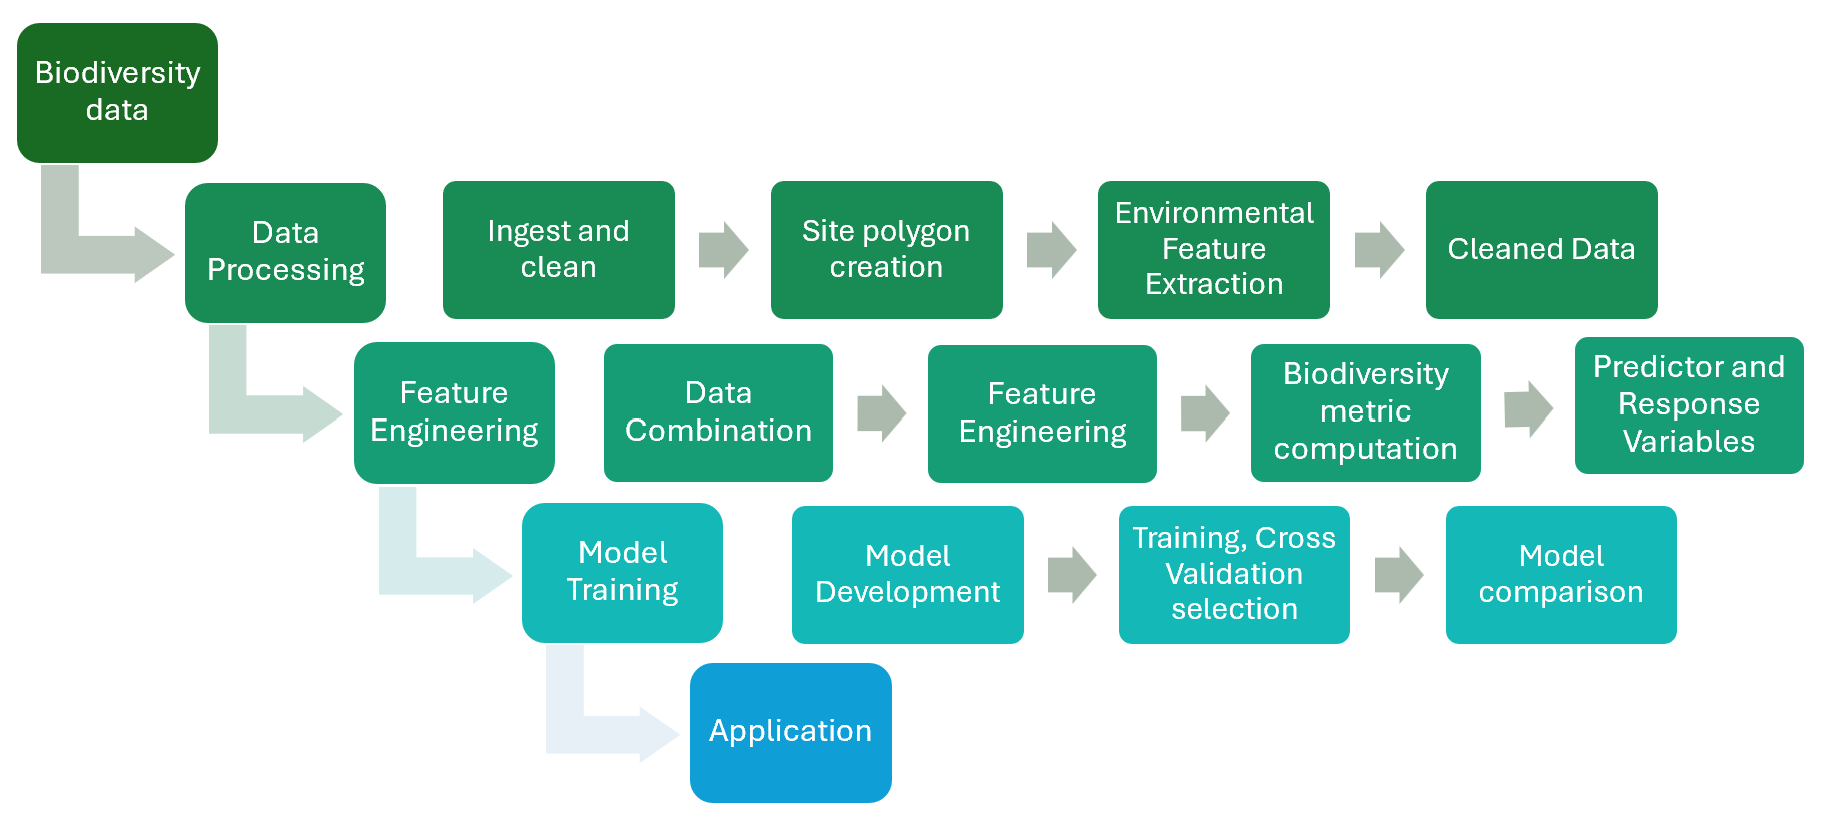
\includegraphics[width=\textwidth]{Images/pipeline_graph.png}
    \caption{Overview of the Spatial Biodiversity Modeling Pipeline (SBM-pipe). The pipeline has 3 main components: data processing, feature engineering, and model training. Each component consists of several steps that are designed to be flexible and adaptable to different types of biodiversity data and modeling approaches. The pipeline is implemented in Python and is available on GitHub \parencite{sbm-pipe}.}
    \label{fig:pipeline_diagram}
\end{figure}

\subsubsection{Biodiversity data input}
The first step in the SBM pipeline is to select appropriate biodiversity data. Researchers can draw on a wide range of biodiversity data sources, including citizen-science initiatives, government-funded monitoring programmes, and researcher-collected datasets \parencite{zipkin2023}; however, to standardize the data input we chose to use the Darwin Core (DwC) format \parencite{wieczorek_darwin_2012}. This format was chosen because it is a flexible and straightforward format for biodiversity data. One of the largest biodiversity data repositories, GBIF, standardizes its data according to this format and the data used specifically to test the SBM pipeline is in Section~\ref{subsec:data}. While this format is widely used, it is important to note that there are many other formats for biodiversity data, and the SBM pipeline is designed to account for this by allowing other formats as long as the user provides a mapping to DwC format. 

\subsubsection{Data Processing}
Once the biodiversity dataset is chosen by the user, the next step in the SBM pipeline is to process the data. This involves several steps, including ingesting and cleaning the data, site polygon creation, and environmental feature extraction. In the ingestion and cleaning step the data is read into the pipeline and any necessary cleaning steps are performed. This includes removing any records with missing or invalid data, removing rows that don't have precise location information, removing records that are outside the dataset's date range, removing exact duplicates, validating location identification integrity, and inferring organism quantity \footnote{GBIF data quality guidance: \url{https://docs.gbif.org/course-data-mobilization/en/data-quality.html} (accessed 2026-05-12).}. Important steps here involve removing rows that are not precise enough for spatial modeling, this includes records whose latitude and longitude values are not precise enough, usually less than four decimal places, and the precision of these values can be specified by the user. Another important step is validating location identification integrity, if a biodiversity dataset is conduct over many decades, it is possible that the same unique location identifier (location ID) may change. This results in many location IDs mapping to the same latitude and longitude values, which can cause issues for spatial modeling. To address this, the pipeline checks for duplicate location IDs on latitude and longitude values and will rename location IDs to ensure that each unique location ID corresponds to a unique latitude and longitude pair. Finally, the pipeline infers organism quantity by checking for the presence of the "individualCount", "organismQuantity", and "organismQuantityType" fields in the dataset which are apart of DwC format \parencite{wieczorek_darwin_2012}. If these fields are not present then the pipeline will infer organism quantity by counting the number of records for each unique location ID, each unique species, and each unique date as sometimes abundance data is not always provided in the default fields. If that data is truly occurrence data (presence/absence) this will have no effect on the dataset. All of these steps can be specified by the user in the configuration file, allowing for flexibility in the data processing step.

After the data is ingested and cleaned, the next step is to create site polygons. This involves creating polygons around each unique latitude and longitude pair in the dataset at different scales. This is done because biodiversity datasets usually vary in spatial scale \parencite{sicacha-parada2022}. The polygons are also created so we can later extract environmental features from these polygons. The user can define the radius for the site polygons as well as the shape of these polygons. If the dataset contains coordinate uncertainty information, then the pipeline will also create polygons with a radius equal to the coordinate uncertainty value. These polygons are projected both in a global coordinate reference system (CRS) and a local CRS, which is determined by the latitude and longitude values of each site. The global CRS, EPSG:4326, is used for extracting environmental features, while the local CRS is used for visualization.

Once every site polygon is created, the next step is to extract environmental features from these polygons. The environmental features are extracted from datasets provided by the user as the choice of environmental features can vary and is not the same for every problem \parencite{williams2012}. The environmental feature datasets should be provided in a raster format, this will allow the SBM pipeline to extract features from the site polygons. The user can also specify the type of summary statistic to use when extracting features from the site polygons, this includes mean, median, min, max, and standard deviation. 

\subsubsection{Feature Engineering}

Once the data has been processed, site polygons created, and environmental features extracted, the next step in the SBM pipeline is to perform feature engineering. The first step in feature engineering is to combine the biodiversity data with the extracted environmental features. This involves joining the biodiversity data with the environmental features based on the unique location ID for each site and time dimension which is usually the year. This results in a dataset that contains both the biodiversity data and the environmental features for each site and time dimension.

Once we have our combined biodiversity and environmental feature dataset, the next step is feature engineering. Feature engineering involves creating new features from the existing data that may be more informative for modeling. This can include creating interaction terms between environmental features, creating polynomial features, or other advanced feature engineering techniques \parencite{Katya2023}. Currently, the feature engineering in the SBM pipeline will log, square, and square root transform the continuous environmental features. 

An important step of the feature engineering process is to calculate the community-level biodiversity metrics that will be used as the target variable for modeling. This includes calculating alpha diversity, which is a measure of the diversity within a single site. Currently the SBM pipeline calculates all the alpha diversity metrics described in Section~\ref{subsec:biodiversity}. This includes species richness, absolute abundance, relative abundance, Shannon index, arithmetic mean abundance, and geometric mean abundance. Furthermore, when calculating these alpha diversity metrics, the user can define the taxonomic resolutions to group at before calculating these metrics. By default no taxonomic grouping done is always included. This type of taxonomic grouping is sometimes used when species-level identification is difficult, costly, or inconsistent \parencite{de_oliveira_higher_2020}. 

At the end of the feature engineering step, we have a datasets that contains community-level biodiversity metrics as well as the environmental features for each site and time dimension and at varying taxonomic resolutions. These datasets can then be used for modeling in the next step of the SBM pipeline.

\subsection{Data}\label{subsec:data}
%Probably go in depth here a
\subsection{Model Selection}\label{subsec:models_selection}
%with evaluation of how a model was chosen and the different models that were considered.
% Go more into the details of the statistical methods?? Focus more on top down methods and the ML methods
\subsection{Model Evaluation Metrics}